\section{Questões de design e implementação}

\begin{frame}
\frametitle{Questões de projeto}
\framesubtitle{Design e implementação}
\begin{itemize}
	\item Algumas questões surgem com o paradigma orientado a objetos
	\item Escolha entre \destaq{flexibilidade} e \destaq{eficiência de execução}
	\item Algumas linguagens focam mais em eficiência que outras
\end{itemize}
\end{frame}

\begin{frame}
\frametitle{Questões de projeto}
\framesubtitle{Exclusividade de Objetos}
\begin{itemize}
	\item Introdução do conceito de classes além dos tipos existentes
	\item \destaq{Vantagens:} uniformidade e elegância
	\item \destaq{Desvantagens:} menor eficiência, pois operações simples são feitas por processos de passsagem de mensagens
\end{itemize}
\end{frame}

\begin{frame}
\frametitle{Questões de projeto}
\framesubtitle{Exclusividade de Objetos}
Escolha entre tipos e classes:
\begin{enumerate}
\item Adição de classes e modelo de objetos à linguagem já existente \texttt{(Objective-C)}
\item Classes são construtores de tipos, ou seja, declarações de classes fazem parte do sistema de tipagem \texttt{(C++)}
\item Exclusão dos outros tipos estruturados, e todos os tipos são classes \texttt{(Smalltalk)}
\end{enumerate}
\end{frame}


\begin{frame}
\frametitle{Questões de projeto}
\framesubtitle{Exclusividade de Objetos}
Exemplos das linguagens:

\begin{itemize}
\item \texttt{Smalltalk}, \texttt{Ruby}: apenas objetos
\item \texttt{C++}, \texttt{Objective-C}, \texttt{Java}, \texttt{C\#}: tipos primitivos + objetos
\end{itemize}
\end{frame}

\begin{frame}
\frametitle{Questões de projeto}
\framesubtitle{Diferenças entre classes e subclasses}

Existem muitas possibilidades de diferenças entre subclasses e classes pai ou base
\begin{itemize}
\item Divergir no número de métodos, parâmetros de algum método, corpo de algum método, tipos de retornos dos métodos diferentes...
\end{itemize}

Normalmente são restringidos:
\begin{itemize}
\item A subclasse restringe-se a um subtipo da classe pai - relacionamentos \destaq{é-um(a)}
\item Métodos da subclasse que sobrescrevem métodos da classe pai devem ser compatíveis com os sobrescritos
\end{itemize}

\end{frame}

\begin{frame}
\frametitle{Questões de projeto}
\framesubtitle{Verificação de tipos e polimorfismo}

Variáveis \destaq{polimórficas} podem referenciar objetos da classe base ou descendentes

\begin{itemize}
	\item Por isso, nem sempre podem ser determinadas estaticamente;
	\item Questão é: sendo dinamicamente, quando realizar as verificações de tipos das vinculações.
\end{itemize}
\end{frame}

\begin{frame}
\frametitle{Questões de projeto}
\framesubtitle{Herança simples e múltipla}

Nas heranças múltiplas, uma nova classe herda duas ou mais classes
\begin{itemize}
	\item Isso pode impactar a linguagem tanto na \destaq{complexidade} de programação quanto na \destaq{eficiência}.
\end{itemize}

\end{frame}

\begin{frame}
\frametitle{Questões de projeto}
\framesubtitle{Herança simples e múltipla}

Exemplo de questão que surge: \destaq{heranças compartilhadas}.

\begin{figure}
	\centering
	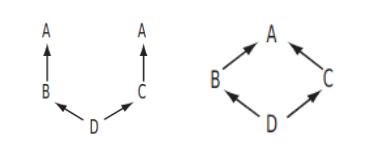
\includegraphics[width=0.7\linewidth]{img/heranca_diamante}
	\caption{A mesma classe pai A é referenciada por B e por C. \cite{louden2012}}
	\label{fig:herancadiamante}
\end{figure}

\begin{itemize}
\item Na esquerda: duas cópias da classe $A$ (herança repetida).
\item Na direita: a mesma cópia de $A$ usada por $B$ e $C$ (herança compartilhada).
\end{itemize}
\end{frame}

\begin{frame}
\frametitle{Questões de projeto}
\framesubtitle{Herança simples e múltipla}
Tipos de herança presentes em algumas linguagens:

\begin{itemize}
	\item \texttt{Smalltalk}: apenas simples
	\item \texttt{Objective-C}: apenas simples, alguns efeitos com protocolos
	\item \texttt{Java}, \texttt{C\#}: apenas simples, alguns efeitos com interfaces
	\item \texttt{Ruby}: apenas simples, alguns efeitos com módulos
	\item \texttt{C++}: ambas
\end{itemize}
\end{frame}

\begin{frame}
\frametitle{Questões de projeto}
\framesubtitle{Vinculação estática e dinâmica}

\begin{itemize}
\item Vinculações estáticas ou dinâmicas;
\item Estáticas são mais rápidas, mas as dinâmicas também possuem vantagens;
\item \destaq{Exemplos em linguagens:}
\item \texttt{Smalltalk}, \texttt{Ruby}: todas as vinculações são dinâmicas
\item \texttt{C++}, \texttt{Objective-C}, \texttt{Java}, \texttt{C\#}: podem ser estáticas ou dinâmicas
\end{itemize}
\end{frame}

\begin{frame}
\frametitle{Questões de projeto}
\framesubtitle{Alocação e liberação de objetos}
\begin{itemize}
\item Memória stack ou heap;
\item Em atribuições de objetos de classes iguais ou descendentes, escolher entre cópia de ponteiros ou valores;
\item Alocação e desalocação implícita ou explícita.
\item \destaq{Exemplos:}
\item \texttt{C++}: os objetos podem ser estáticos, dinâmicos na stack ou dinâmicos na heap;  alocações e desalocações são feitas explicitamente.
\item \texttt{Java}: objetos são dinâmicos na heap; alocação é explícita e desalocação é implícita.
\end{itemize}
\end{frame}


\begin{frame}[fragile]
\frametitle{Questões de projeto}
\framesubtitle{Classes aninhadas}
Caso uma classe seja utilizada apenas por uma outra, pode-se escolher \destaq{ocultá-la} das outras. Exemplo:

\begin{verbatim}
class Arvore {
   class No {
      ...
   };

   std::vector<No> nos;
   ...
};
\end{verbatim}

\begin{itemize}
\item Existem em \texttt{C++}, \texttt{Java}, \texttt{C\#}, \texttt{Ruby}, mas não em \texttt{Smalltalk} e \texttt{Objective-C}.
\end{itemize}

\end{frame}


\begin{frame}
\frametitle{Questões de projeto}
\framesubtitle{Inicialização de objetos}

\begin{itemize}
\item Pode-se optar por inicializar objetos manualmente ou por algum mecanismo implícito;
\item Em objetos de subclasse, pode-se associar a inicialização à classe pai ou não
\item \destaq{Exemplos:}
\item \texttt{C++}, \texttt{Java}, \texttt{C\#}, \texttt{Ruby}: construtores são chamados implicitamente;
\item \texttt{Smalltalk} e \texttt{Objective-C}: construtores são chamados explicitamente.
\end{itemize}
	
\end{frame}

